\section{Introduction}
\label{sec:intro}

Time series data represents the temporal pulse of our interconnected physical, biological, and socio-economic systems. Over the past several decades, the study of temporal sequence modeling has evolved across three major technological waves: classical statistical and autoregressive modeling (e.g., ARIMA, exponential smoothing), task-specific deep neural architectures (e.g., RNNs, LSTMs, TCNs, Informer, PatchTST), and most recently, large pre-trained Time Series Foundation Models (TSFMs)~\cite{Goswami2024MOMENT,Liu2024Timer,Ansari2024Chronos,Ekambaram2024TTM}. 

Despite extraordinary advances in univariate and multivariate numerical modeling, an essential constraint persists across unimodal paradigms: \textit{real-world temporal dynamics do not unfold in an informational vacuum}. When a sudden traffic congestion spike occurs, an electrical grid frequency deviates, or a stock price undergoes rapid volatility, the underlying generative causes are rarely confined to historical numerical values alone. Instead, these phenomena are profoundly shaped by external multimodal signals: breaking news reports, meteorological alerts, natural language operational dispatches, visual monitoring streams, and relational graph topologies. 

\begin{figure*}[t]
\centering
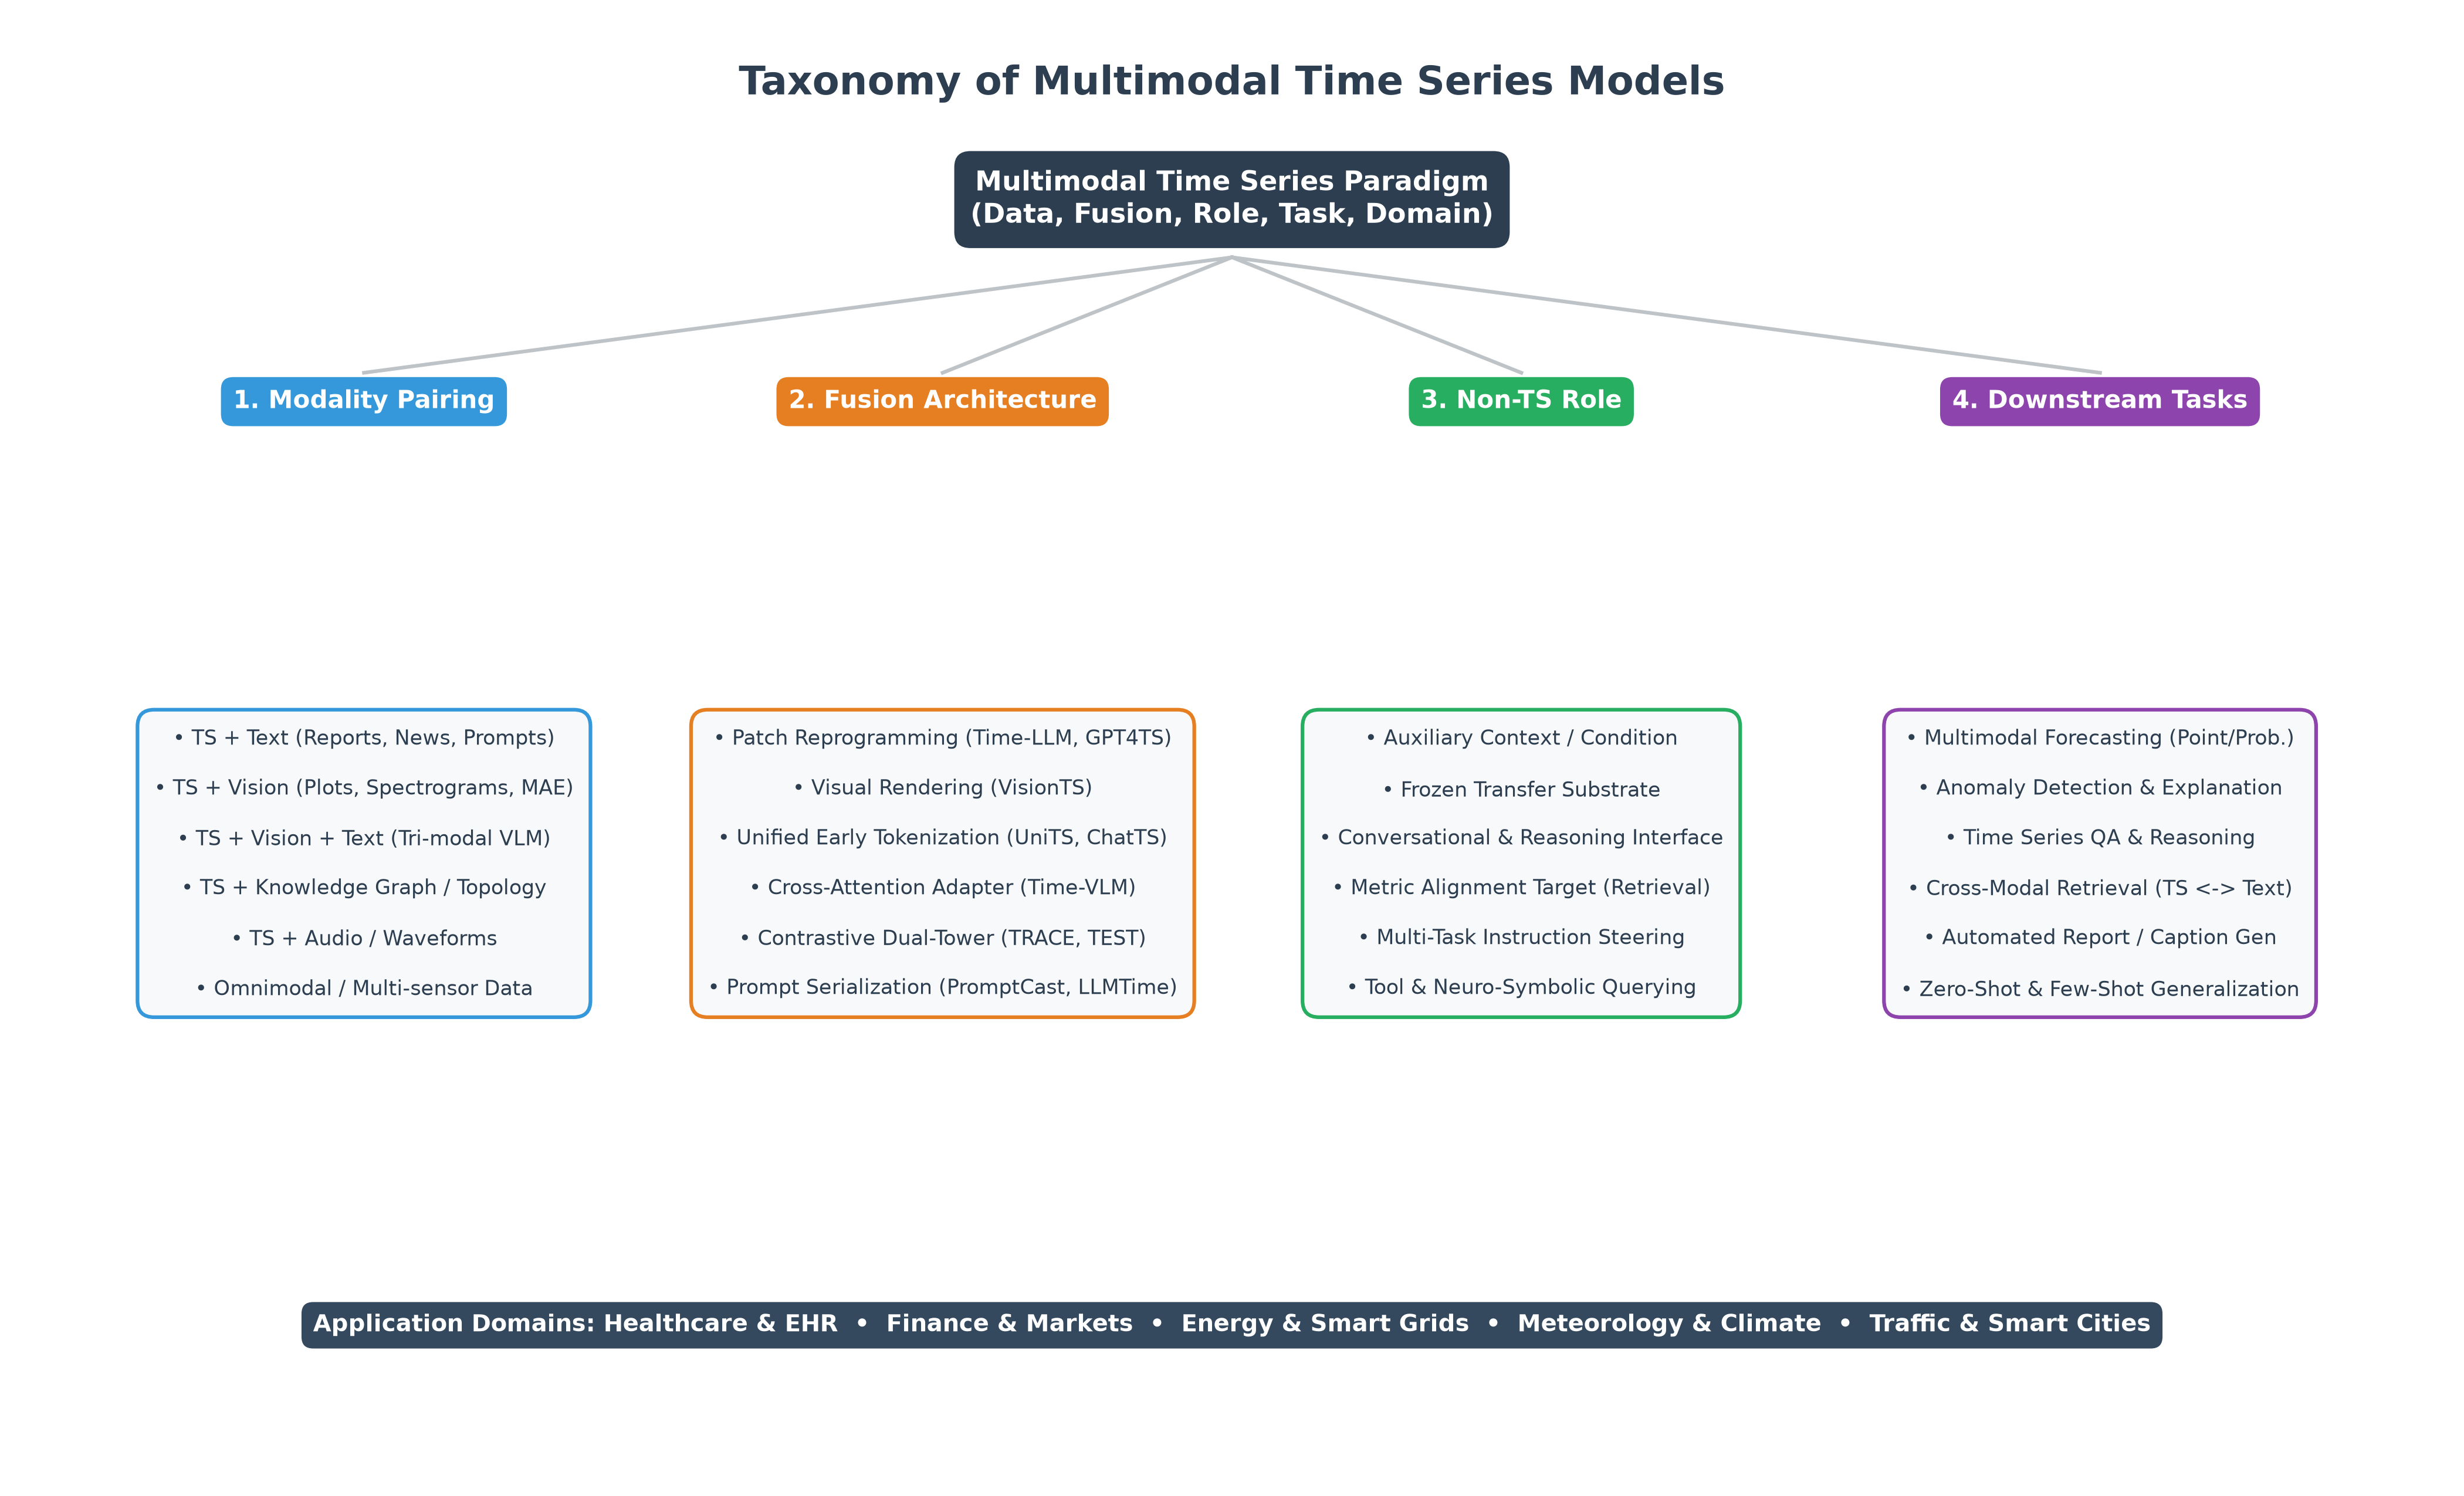
\includegraphics[width=0.98\textwidth]{figures/taxonomy.png}
\caption{The proposed multidimensional taxonomy for multimodal time series models, organizing the literature across four core pillars: Modality Pairing, Fusion Architecture, Role of the Complementary Modality, and Downstream Predictive/Analytical Tasks across diverse application domains.}
\label{fig:taxonomy}
\end{figure*}

\subsection{The Rise of Multimodal Time Series Intelligence}
The unprecedented general reasoning capabilities of pre-trained Large Language Models (LLMs) and Vision-Language Models (VLMs) have fundamentally transformed artificial intelligence. Researchers quickly observed that the sequence modeling principles governing language and vision exhibit deep mathematical parallels with time series. This has catalyzed an explosion of research exploring the intersection of time series and multimodal models:
\begin{enumerate}
    \item \textbf{Cross-Modal Reprogramming:} Groundbreaking frameworks such as Time-LLM~\cite{Jin2023TimeLLM} and One Fits All (GPT4TS)~\cite{Zhou2023OneFitsAll} demonstrated that frozen language model backbones (e.g., GPT-2, LLaMA) can be repurposed as high-accuracy time-series forecasters by patching time series and aligning temporal representations with textual semantic prompts.
    \item \textbf{Visual Transcoding \& Vision-Language Synergy:} Counter-intuitively, VisionTS~\cite{Chen2024VisionTS} revealed that reformulating numeric series as line-chart images allows off-the-shelf visual masked autoencoders (MAE pre-trained on ImageNet) to perform competitive zero-shot forecasting without any domain fine-tuning. Concurrently, Time-VLM~\cite{Zhong2025TimeVLM} unites visual, textual, and temporal representations for augmented forecasting.
    \item \textbf{Conversational Reasoning \& TS-MLLMs:} Pioneering systems such as ChatTS~\cite{Zhao2024ChatTS}, TimeOmni-1~\cite{Tan2025TimeOmni1}, and ChatTime~\cite{ChatTime2024} elevate time-series models from passive function approximators to interactive reasoning agents capable of answering temporal questions, conducting counterfactual reasoning, and explaining anomalies.
    \item \textbf{Multimodal Datasets \& Benchmarks:} Systematic benchmarks such as Time-MMD~\cite{Liu2024TimeMMD}, Fidel-TS~\cite{FidelTS2025}, and MTBench~\cite{MTBench2025} have begun curating high-fidelity, aligned cross-modal time series corpora across diverse real-world domains.
\end{enumerate}

\begin{table*}[t]
\caption{Comparison of This Survey with Existing Surveys in Time Series and Large Models.}
\label{tab:survey_comparison}
\centering
\small
\resizebox{\textwidth}{!}{%
\begin{tabular}{lcccccc}
\toprule
\textbf{Survey Reference} & \textbf{Year} & \textbf{Scope Focus} & \textbf{TS Modalities} & \textbf{Cross-Modal Fusion} & \textbf{TS-MLLM Reasoning} & \textbf{PRISMA Protocol} \\
\midrule
Jin et al.~\cite{Jin2023LargeModelsSurvey} & 2023 & Large Models (TS \& ST) & TS + Spatio-Temporal & Partial & Limited & No \\
Jin et al.~\cite{Jin2024PositionLLMTS} & 2024 & Position: LLMs for TS & Numerical TS & Reprogramming focus & Preliminary & No \\
\textbf{This Survey} & \textbf{2026} & \textbf{Multimodal TS Models} & \textbf{TS + Text + Vision + KG} & \textbf{Comprehensive} & \textbf{In-Depth (2021--2026)} & \textbf{Yes (PRISMA 2020)} \\
\bottomrule
\end{tabular}%
}
\end{table*}

\subsection{Need for a Dedicated Survey}
While prior comprehensive surveys have examined large foundation models for pure time-series or spatio-temporal data~\cite{Jin2023LargeModelsSurvey,Jin2024PositionLLMTS}, they predominantly focus on unimodal foundation architectures or single-modality adaptation. As shown in \Cref{tab:survey_comparison}, there lacks a dedicated, systematic survey synthesizing the rapid evolution of \textit{explicitly multimodal time series modeling}—spanning text-guided forecasting, vision-based time series modeling, multi-task unified architectures, and conversational reasoning agents.

\subsection{Contributions of This Survey}
To fill this critical void, this paper provides:
\begin{itemize}
    \item \textbf{A Systematic, Verifiable Review:} Conducted under the PRISMA 2020 framework spanning 2021 to 2026, where every cited paper is verified against authoritative bibliographic APIs.
    \item \textbf{A Four-Pillar Taxonomy:} A taxonomy deconstructing multimodal time series research along Modality Pairing, Fusion Architecture, Non-TS Role, and Downstream Tasks (\Cref{fig:taxonomy}).
    \item \textbf{Deep Methodological Analysis:} A unified comparative dissection of cross-modal reprogramming, visual line-chart transcoding, contrastive alignment, and interactive reasoning architectures.
    \item \textbf{Curated Resource \& Dataset Landscape:} An exhaustive mapping of multimodal benchmark datasets, open-source repositories, and evaluation protocols.
    \item \textbf{Critical Perspectives on Open Challenges:} A rigorous appraisal of the modality gap, benchmark data contamination, temporal granularity mismatches, and future research trajectories.
\end{itemize}
